\section{Protection des variables}
La protection des variables permet de ne pas accéder à une ressource commune à plusieurs processus en même temps. C'est donc tout naturellement qu'on devrait protéger chaque moyen de communication mis en place. En réalité, la file de message contenant les requetes des bus ne nécessite pas de protection car un processus se charge de créer les bus et un autre consomme l'information directement pour changer le feu. Il faut néanmoins protéger les feux. Pour cela, un sémaphore est nécessaire afin de ne pas changer un feu en même temps qu'une voiture consulte son état ce qui donnerait un résultat totalement aléatoire. Un second sémaphore est nécessaire pour gérer les voies de sortie. En effet, à chaque changement de feu, les voies de sortie sont mises à 0 et sont consultées en permanence lors d'un passage de voiture. Encore une fois, pour éviter un résultat aléatoire, celui-ci est nécessaire. Enfin, un dernier mutex est nécessaire pour signaler le changement de feu.

\begin{figure}[htb!]
\centering
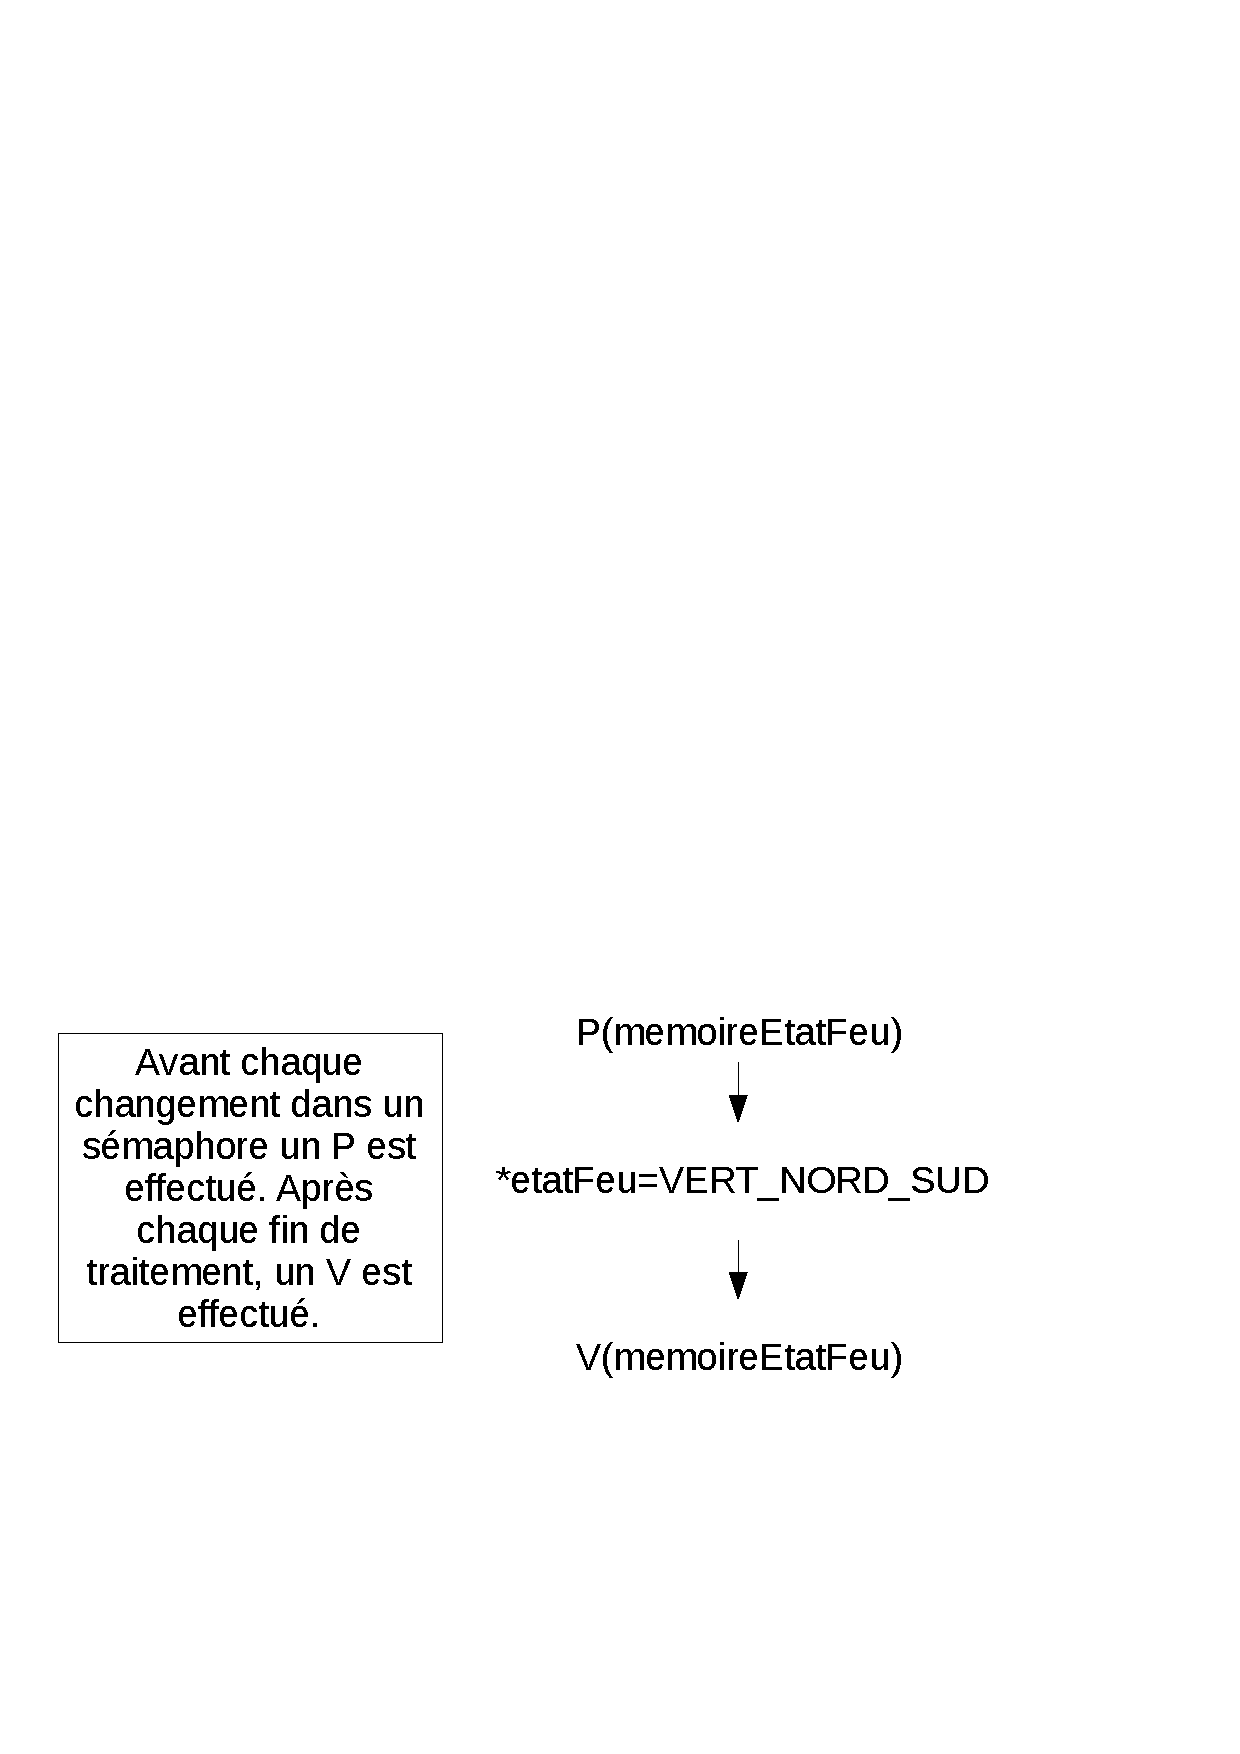
\includegraphics[scale=0.5]{graphe2LO41.pdf}

\caption{Utilisation des sémaphores}
\end{figure}
